\section{}
A gas is contained in a vertical, frictionless piston-cylinder device. The piston has a mass 
of 5 kg and a cross-sectional area of 35 cm$^2$. A compressed spring above the piston exerts a 
force of 75 N on the piston. If the atmospheric pressure is 95 kPa, determine the pressure inside 
the cylinder.

\begin{figure}[h]
    \centering
    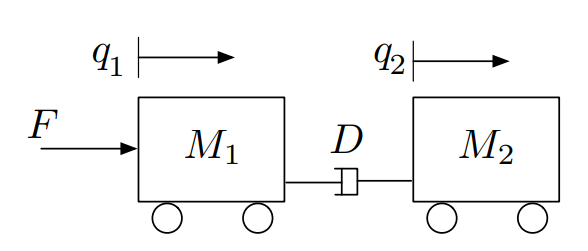
\includegraphics[width=0.5\textwidth]{Questions/Figures/Q2ProblemDiagram.png}
    \caption{Piston-cylinder device}
    \label{fig:Q2ProblemDiagram}
\end{figure}
